%%%%%%%%%%%%%%%%%%%%%%%%%%%%%%%%%%%%%%%%%%%%%%%%%%%%%%%%%%%%%%%%%%%%%%%%%%%%%%%%%%%
% Thiago Pelizoni
%%%%%%%%%%%%%%%%%%%%%%%%%%%%%%%%%%%%%%%%%%%%%%%%%%%%%%%%%%%%%%%%%%%%%%%%%%%%%%%%%%%
% Pós-graduação em Engenharia de Software - Universidade São Judas Tadeu - São Paulo - SP
%%%%%%%%%%%%%%%%%%%%%%%%%%%%%%%%%%%%%%%%%%%%%%%%%%%%%%%%%%%%%%%%%%%%%%%%%%%%%%%%%%

%%%%%%%%%%%%%%%%%%%%%%%%%%%%%%%%%%%%%%%%%%%%%%%%%%%%%%%%%%%%%%%%%%%%%%%%%%%%%%%%%%%
% Trabalho referente a matéria de Métricas de Software
%%%%%%%%%%%%%%%%%%%%%%%%%%%%%%%%%%%%%%%%%%%%%%%%%%%%%%%%%%%%%%%%%%%%%%%%%%%%%%%%%%%

\documentclass[11pt, a4paper]{article}				

\usepackage[utf8]{inputenc}
\usepackage[brazil]{babel}	
\usepackage{graphicx,color}
\usepackage[left=1.5cm,top=2.0cm,right=1.5cm,bottom=1.5cm]{geometry}
\usepackage{enumerate}
\usepackage{epigraph}
\usepackage{abntcite}
\usepackage{float}
\usepackage{amsmath}

% Título do trabalho
\title{Uso de métricas de software na quantificação dos custos de erros encontrados em um projeto real}

% Autor
\author{
	Thiago Pelizoni \\
	André Terceiro \\
	Rodrigo Raminelli \\
	Pedro A. Saraiva Junior
}

\date{2013}


%%%%%%%%%%%%%%%%%%%%%%%%%%%%%%%%%%%%%%%%%%%%%%%%%%%%%%%%%%%%%%%%%%%%%%%%%%%%%%%%%%%

\begin{document}

% Faz a criação do título do documento
\maketitle

%%%%%%%%%%%%%%%%%%%%%%%%%%%%%%%%%%%%%%%%%%%%%%%%%%%%%%%%%%%%%%%%%%%%%%%%%%%%%%%%%%%
% Resumo
%%%%%%%%%%%%%%%%%%%%%%%%%%%%%%%%%%%%%%%%%%%%%%%%%%%%%%%%%%%%%%%%%%%%%%%%%%%%%%%%%%%
\begin{abstract}
O custo de defeitos em software tende a crescer exponencialmente a medida que as etapas do desenvolvimento de software avançam. O valor pode ser alto ao ponto de custar entre 90 a 880 vezes o valor do levantamento deste requisito na sua fase inicial.\cite[p. 37]{NISL} A Engenharia de Software utiliza métricas de produto afim de construir um software de alta qualidade. Desta forma, este trabalho tem o intuito de demonstrar a aplicação das técnicas de métricas de software no projeto de inscrição dos participantes da Corrida de São Silvestre afim de quantificar os erros encontrados, seja na fase de testes, homologação ou produção e calcular o custo destes erros, evidenciando o quanto a empresa economizaria em uma melhoria no processo.


\end{abstract}


%%%%%%%%%%%%%%%%%%%%%%%%%%%%%%%%%%%%%%%%%%%%%%%%%%%%%%%%%%%%%%%%%%%%%%%%%%%%%%%%%%%
% 1. Introdução
%%%%%%%%%%%%%%%%%%%%%%%%%%%%%%%%%%%%%%%%%%%%%%%%%%%%%%%%%%%%%%%%%%%%%%%%%%%%%%%%%%%
% Descreve porquê o trabalho foi feito.
\section{Introdução}
São comuns abordagens a respeito de qualidade de software, que é necessário seguir boas práticas para se obter um software de alta qualidade, no entanto, como pode ser definida a qualidade? Em um sentido geral, qualidade de software é a satisfação de requisitos funcionais e de desempenho explicitamente declarados, normas de software explicitamente documentadas e características implícitas que são esperadas em todo o software desenvolvido profissionalmente. A partir desta definição, podem ser enfatizados três pontos importantes:

\begin{enumerate}
	\item Requisitos de software são a fundação a partir da qual a qualidade é medida. A falta de conformidade com os requisitos é falta de qualidade.
	\item Normas especificadas definem um conjunto de critérios de desenvolvimento que guiam o modo pelo qual o software é construído. Se os critérios não são seguidos, quase sempre, irá resultar em falta de qualidade.
	\item Há um conjunto de requisitos implícitos que frequentemente não são mencionados, por exemplo, o desejo de facilidade de uso (usabilidade). Se os software satisfaz os requisitos explícitos, mas deixa de satisfazer requisitos implícitos, a qualidade do software é suspeita.
\end{enumerate}
\cite[p.349]{pressman}

\subsection{Métricas de Software}
\epigraph{A qualidade de um produto é função de quanto ele muda o mundo para melhor}{Tom DeMarco\cite[p.350]{pressman}}

Um elemento-chave que a engenharia utiliza em seu processo é a medição, de modo a ter um melhor entendimento dos atributos dos modelos criados afim de avaliar a qualidade seus produtos ou sistemas desenvolvidos.

De acordo com Pressman, a medição é um processo pelo qual números ou símbolos são associados aos atributos de entidades do mundo real, de modo que os determinem de acordo com regras claramente definidas. Nas ciências físicas, medicina, economia e mais recentemente nas ciências sociais, atualmente é possível medir atributos que anteriormente não eram mensuráveis. Obviamente, tais medições em engenharia de software não são tão refinadas quanto muitas medições nas ciências físicas mas, elas existem e decisões importantes são tomadas com base nelas. A obrigação de tentar medir o não mensurável afim de melhorar o entendimento de entidades particulares é tão potente em engenharia de software como em qualquer outra disciplina.\cite[p.348]{pressman}

\subsubsection{Medidas, Métricas e Indicadores}
\epigraph{Uma ciência é tão madura quanto seus instrumentos de medição}{Louis Pasteur\cite[p.352]{pressman}}

Em engenharia de software, uma medida fornece uma indicação quantitativa da extensão, qualidade, dimensão, capacidade ou tamanho de algum produto ou processo, deste modo, podemos definir como \textit{medição} o ato de determinar uma medida.\cite[p.348]{pressman}

Quando um ponto de dados é coletado, por exemplo, o número de erros descoberto em um componente de software, uma medida é estabelecida. Neste caso, a medição ocorre como o resultado da coleção de um ou mais ponto de dados, por exemplo, um certo número de revisões de componentes e testes de unidade são investigados afim de coletar medidas do número de erros de cada um.

Uma métrica de software visa relacionar as medidas individuais de algum modo, por exemplo, o número de erros encontrados por revisão ou o número médio de erros encontrados por teste de unidade. Com posse dessas informações, um engenheiro de software desenvolve métricas de modo que os indicadores possam ser obtidos. Um \textit{indicador} consiste em um \textit{métrica} ou em uma combinação de \textit{métricas} cujo intuito é fornecer uma profundidade na visão do processo de software, projeto de software ou o produto em si.\cite{pressman}

\subsubsection{Princípios de Medição}
De acordo com Pressman um processo de medição pode ser caracterizado por cinco atividades:

\begin{enumerate}
	\item \textit{Formulação}: A derivação de medidas e métricas de software adequadas para a representação do software que está sendo considerado.
	\item \textit{Coleta}: Mecanismo usado para acumular os dados necessários para derivar as métricas formuladas.
	\item \textit{Análise}: Cálculo de métricas e aplicação das ferramentas matemáticas.
	\item \textit{Interpretação}: Avaliação das métricas em um esforço para ganhar profundidade na visão da qualidade da representação.
	\item \textit{Realimentação}: Recomendações derivadas da interpretação das métricas de produto transmitidas à equipe de software.
\end{enumerate}
\cite[p.353]{pressman}

\subsection{Objetivo deste trabalho}
Tendo por base as informações anteriormente citadas, o objetivo deste trabalho demonstrar a aplicação das técnicas de métricas no projeto de inscrição dos participantes da Corrida de São Silvestre, afim de quantificar os erros encontrados, sejam estes na fase de testes, homologação ou produção; calcular o custo destes erros afim evidenciar o quanto a empresa economizaria em uma melhoria no processo, detectando os erros em fases do processo de desenvolvimento em que tal detecção é menos onerosa em termos financeiros.


%%%%%%%%%%%%%%%%%%%%%%%%%%%%%%%%%%%%%%%%%%%%%%%%%%%%%%%%%%%%%%%%%%%%%%%%%%%%%%%%%%%
% 2. Materiais e métodos – como foi feito?
%%%%%%%%%%%%%%%%%%%%%%%%%%%%%%%%%%%%%%%%%%%%%%%%%%%%%%%%%%%%%%%%%%%%%%%%%%%%%%%%%%%
% – Referencial teórico
\section{Materiais e métodos}

\subsection{Melhoria de processo}
As medições de um processo de software são dados quantitativos quanto ao mesmo, desta forma, a medição de seus atributos é algo essencial para o seu aprimoramento \cite[p.446]{sommerville}.

De acordo com Sommerville, há um elo entre a qualidade do processo de desenvolvimento com a qualidade do produto que está sendo desenvolvido \cite[p.440]{sommerville}. 

Diante deste fato, a simples adoção de uma metodologia de desenvolvimento utilizada em uma determinada organização ou, o uso de ferramentas não garantem a melhoria do processo desejada. O aprimoramento do processo é uma atividade cíclica constituído de três estágios, são eles:

\begin{itemize}
	\item \textit{Medição}: São medidos os atributos de um projeto da organização ou de seu produto atual.
	\item \textit{Análise}: O projeto vigente é avaliado de modo a identificar seus pontos fortes e fracos.
	\item \textit{Mudança}: São efetuadas mudanças de acordo com as informações obtidas na fase de análise.
\end{itemize}
\cite[p.441]{sommerville}

Nesta sessão será descrito todo o processo de desenvolvimento de software da Fundação Casper Líbero tendo como estudo de caso o projeto de inscrição dos participantes da corrida de Sao Silvestre. Será detalhado o papel de cada profissional de acordo com a etapa do processo e, será aplicada a abordagem GQM\footnote{Goal Question Metrics} afim de especificar um objetivo para a medição e, através de questões bem formuladas, obter as métricas necessárias para atingir o objetivo proposto afim de analisar os dados e propor as mudanças necessárias para a melhoria do processo.

\subsection{O projeto}
O projeto ao qual foi estudo de caso descrito neste artigo, como dito anteriormente, foi o de inscrição dos participantes da corrida de Sao Silvestre desenvolvido pela Fundação Casper Líbero. Este projeto conta com mais de 150.000 linhas de de código. A linguagem de programação utilizada é PHP\footnote{PHP é uma linguagem de programação interpretada, livre, usada originalmente apenas para o desenvolvimento de aplicações server-side, capazes de gerar conteúdo dinâmico na Web.} na versão 5.3.18, Zend Framework 1.12\footnote{Zend Framework é um framework para aplicações Web de código aberto implementado em PHP 5 completamente orientado a objetos,  licenciado sob a New BSD License.}, banco de dados Oracle, controlador de versão Git\footnote{Git é um sistema de controle de versão distribuído projetado e desenvolvido por Linus Torvalds.} e o Trello\footnote{Trello é um organizador de tarefas e eventos bastante dinâmico e funcional, bastante utilizado para gerenciar projetos com a metodologia Scrum.} para gerenciamento das atividades.

O projeto citado havia sido criado em 2012 porém, passou por diversas modificações arquiteturais, visuais e melhorias em geral de modo a englobar novas regras de negócio bem como, correções de problemas identificado na versão anterior.

\subsection{Testes}
O projeto não conta com testes unitários. Os testes em sua maioria são efetuado pelos analistas de negócio do produto de maneira manual. Afim automatizar estes testes manuais, uma bateria de testes do sistema foram criados utilizando o Selenium IDE\footnote{Selenium IDE é um ambiente integrado de desenvolvimento para scripts de testes automatizados simulando o comportamento de um usuário.}. Desta forma, a cada nova funcionalidade criada ou, correção efetuada, estes testes são rodados pelo desenvolvedor. Todavia, os responsáveis pela homologação efetuam os testes manualmente.

\subsection{Gerenciamento do processo de desenvolvimento}
A empresa não segue uma metodologia de desenvolvimento de mercado, por exemplo, Scrum, RUP, etc. Trata-se de um desenvolvimento incremental onde, cada funcionalidade é especificada, desenvolvida, testada e colocada em produção.

\subsubsection{Board do projeto}

Como dito anteriormente, a empresa utiliza-se do Trello para o gerenciamento das atividades de um projeto. Cada projeto refere-se unica e exclusivamente a um board\footnote{O board de um projeto no Trello é o equivalente a Kanban online, conforme pode ser observado na figura "Board das tarefas do projeto".}, de modo a não misturar informações com outros projetos. Na figura a seguir podemos observar o board do projeto mencionado por este artigo.

\begin{figure}[H]
  \caption{Board das tarefas do projeto}
  \centering 
  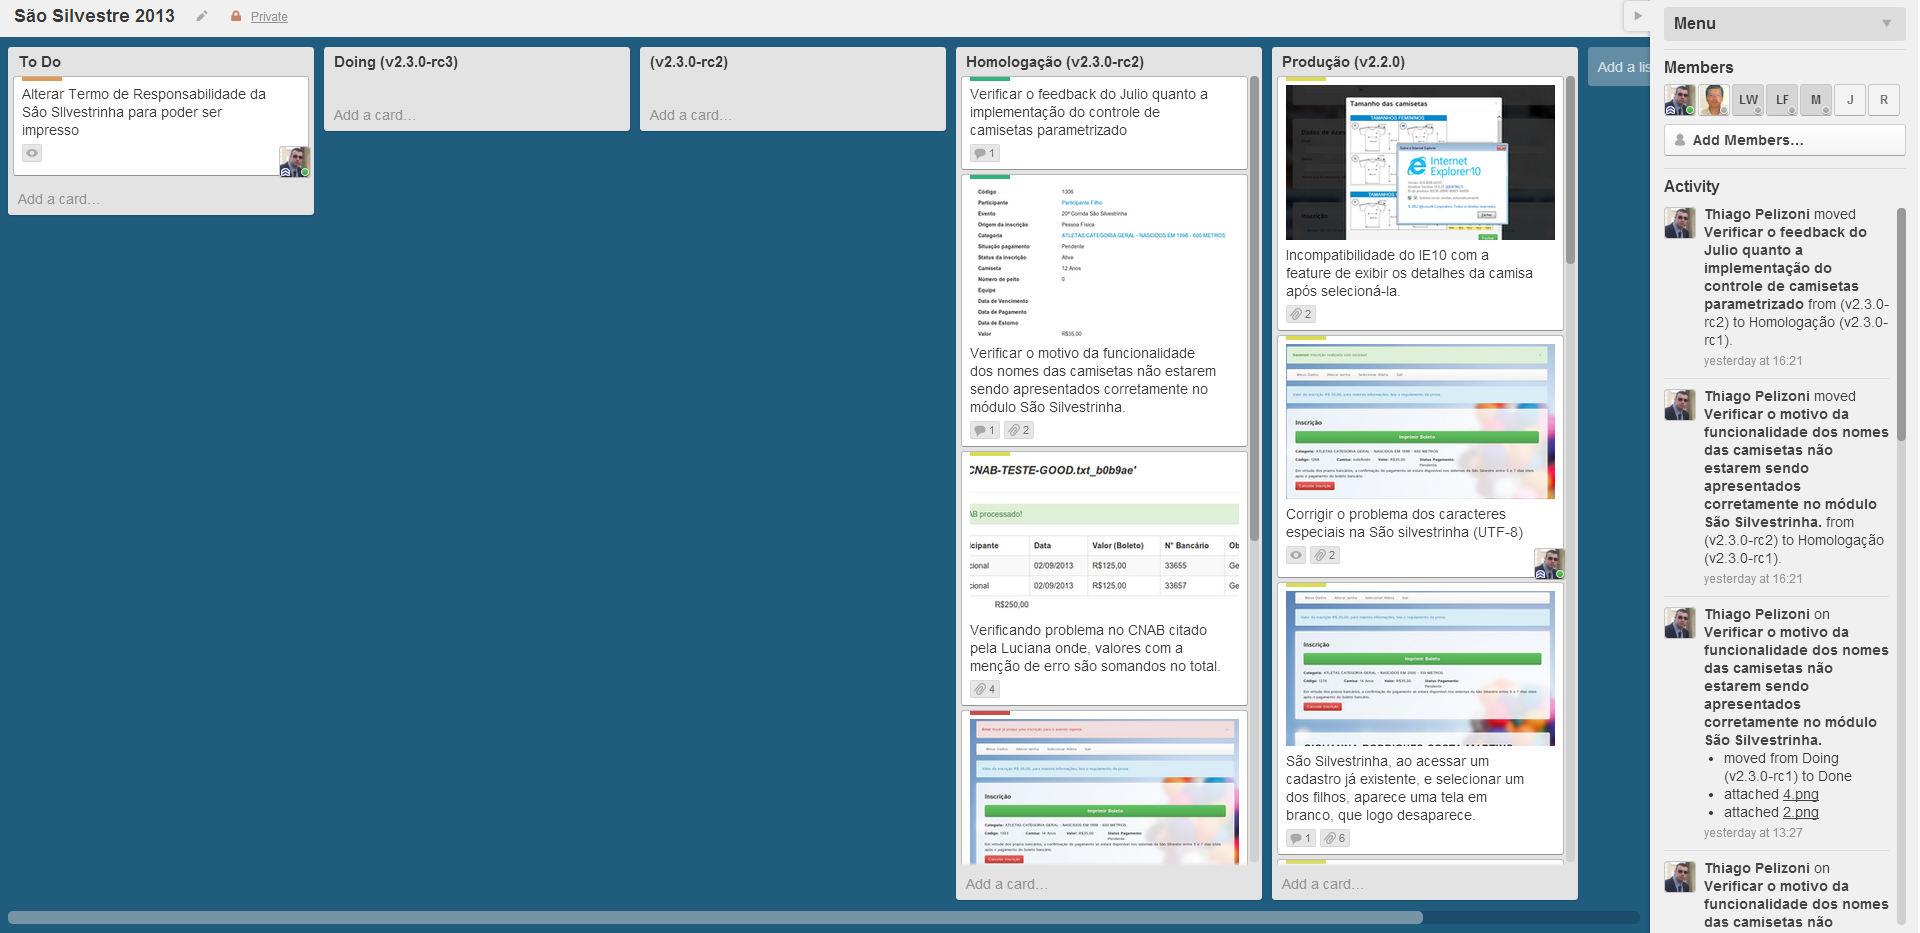
\includegraphics[width=160mm,height=90mm]{images/board.png}
\end{figure}

Cada coluna do board representa um estágio da tarefa onde, este board está dividido em cinco colunas, sendo elas:

\begin{itemize}
	\item \textit{To do}: Refere-se a todas as tarefas que necessitam ser feitas. Primeiras tarefas da coluna possuem maior prioridade.
	\item \textit{Doing}: Refere-se as tarefas que estão sendo feitas em um determinado momento. Cada programador pode ter apenas uma tarefa sendo feito em um dado momento. Quando algum item com maior prioridade, como por exemplo, um defeito em produção, o programador coloca sua tarefa novamente na coluna "To do", traz a tarefa que diz respeito ao problema para a coluna "Doing" e realiza a correção.
	\item \textit{Done}: Refere-se as tarefas que foram concluídas. Estas tarefas, após testadas pelo desenvolvedor e evidenciadas que estão de acordo com o especificado, estarão aptas para serem homologadas por quem solicitou tal tarefa.
	\item \textit{Homologação}: Referem-se as tarefas que encontram-se em ambiente de homologação sendo analizadas pelos solicitantes. Caso haja um problema, uma tarefa com o rótulo de "Correção" será criado na coluna "To do", e passará pelo processo descrito anteriormente. Caso as tarefas estejam de acordo, estas estarão áptas para irem para a produção.
	\item \textit{Produção}: Referem-se as tarefas que foram homologadas pelos solicitantes, geralmente, os analistas de negócios. Quando um problema em produção é encontrado, a tarefa criada faz referência a tarefa na coluna de produção, afim de manter um histórico.
\end{itemize}

\subsubsection{Tarefas}

Toda e qualquer nova tarefa, seja uma nova funcionalidade, alteração ou correção de bugs encontrados, independente do ambiente ao qual este se encontra, é gerado um card\footnote{Um card nada mais é do que uma tarefa dentro do board do Trello.} no Trello.

\begin{figure}[H]
  \caption{Uma tarefa do projeto}
  \centering 
  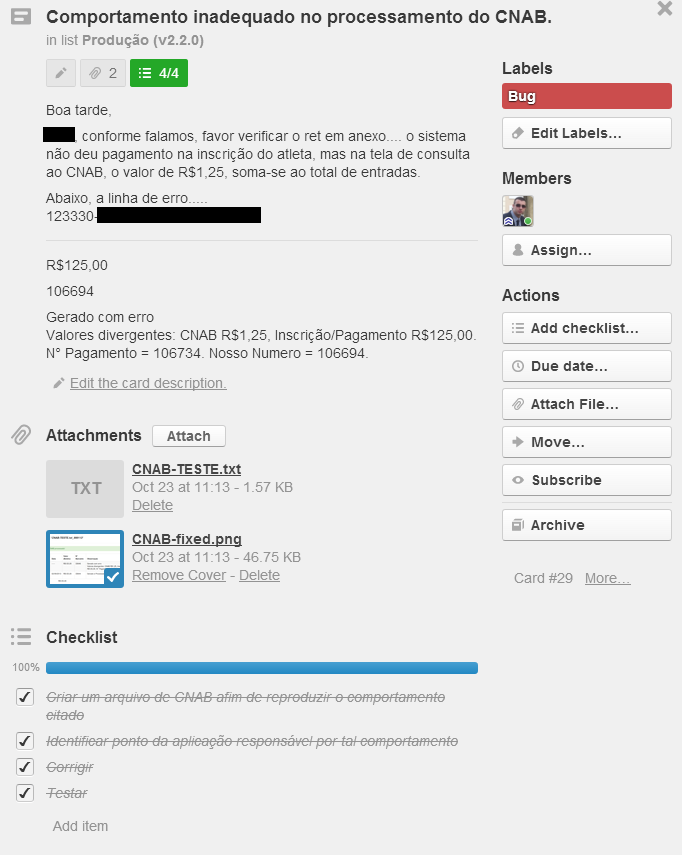
\includegraphics[width=150mm,height=180mm]{images/card.png}
\end{figure}

Como pode ser observado acima, uma tarefa segue uma estrutura básica:
\begin{itemize}
	\item \textit{Título}: Uma breve descrição da tarefa a ser realizada.
	\item \textit{Descrição}: Uma descrição detalhada da tarefa a ser realizada.
	\item \textit{Rótulo}: Qual é o tipo da tarefa.
	\item \textit{Membros}: Quem é o responsável por esta tarefa. Pode haver mais de uma pessoa dependendo do caso, por exemplo, um desenvolvedor e um analista de negócios.
	\item \textit{Checklist}: Quais os passos necessários para a conclusão da tarefa, afim de mensurar em quantos por cento esta atividade se encontra quando em execução.
	\item \textit{Anexos}: Evidências de que a funcionalidade ou as correções estão de acordo com o especificado. Em grande parte dos casos são screenshots.
\end{itemize}

\subsubsection{Rótulo para as tarefas}

Cada tarefa possui um rótulo, de modo a ficar mais fácil identificar o que cada tarefa é através de cores. Desta forma, ao olhar o board de modo geral, através dessas cores é possível identificar e reordenar as tarefas de acordo com sua prioridade de maneira mais fácil.

\begin{figure}[H]
  \caption{Rótulos das tarefas}
  \centering 
  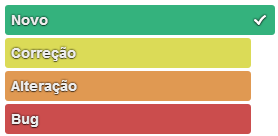
\includegraphics{images/labels.png}
\end{figure}

Como pode ser observado na imagem acima, atualmente, as tarefas podem ser de quatro tipos diferentes:

\begin{itemize}
	\item \textit{Novo}: Refere-se a alguma nova funcionalidade na aplicação.
	\item \textit{Correção}: Refere-se a correção de algum problema identificado no processo de homologação de uma funcionalidade, por exemplo, se uma funcionalidade foi implementada porém, ao verificá-la constatou-se um problema, um card com este rótulo será aberto para a devida correção.
	\item \textit{Alteração}: Refere-se a alteração de alguma funcionalidade na aplicação.
	\item \textit{Bug}: Refere-se a um problema encontrado em ambiente de produção. Geralmente estas tarefas em mais prioridade do que as demais.
\end{itemize}

\subsection{Indicadores}
Conforme descrito no processo de desenvolvimento, todas as informações referente ao gerenciamento do projeto encontram-se na ferramenta Trello. Todavia, há alguns meses, o responsável pela equipe de desenvolvimento foi desligado da empresa e, uma enorme quantidade de informações do projeto São Silvestre foi perdido contendo toda a base histórica do projeto do ano de 2012 e uma boa quantidade das informações do projeto de 2013 pois, o board do projeto estava atrelado a conta pessoal deste funcionário e não da empresa. 

Uma tarefa pode conter um ou vários commits para sua conclusão. Isto muitas vezes deve-se a complexidade da mesma. Para toda e qualquer tarefa, um novo \textit{branch} é criado afim de isolar ela da linha principal enquanto tal funcionalidade não estiver homologada afim de fazer parte da linha principal da aplicação, o branch \textit{master}.

Desta forma, além do board do projeto São Silvestre atual, o histórico de commits do repositório do projeto no BitBucket\footnote{BitBucket é um serviço gratuito de hospedagem de projetos de software que utilizam Git ou Mercurial como controle de versão. https://bitbucket.org/} será utilizado afim de levantar informações precisas para este trabalho, desde de o começo do desenvolvimento deste até sua versão mais atual \textbf{2.4.0}.

%%%%%%%%%%%%%%%%%%%%%%%%%%%%%%%%%%%%%%%%%%%%%%%%%%%%%%%%%%%%%%%%%%%%%%%%%%%%%%%%%%%
% 3. Resultados – o que foi observado?
%%%%%%%%%%%%%%%%%%%%%%%%%%%%%%%%%%%%%%%%%%%%%%%%%%%%%%%%%%%%%%%%%%%%%%%%%%%%%%%%%%%
\section{Resultados}\label{sec:resultados}
\subsection{Goal Question Metrics}
A técnica \textit{Goal Question Metrics} consiste em um método simples para planejar medições de forma que estas sejam baseadas em objetivos específicos. Portanto, iremos descrever quais foram os objetivos dessas medições bem como, iremos discorrer a respeito dos resultados encontrados.\cite[p.444]{sommerville}

\subsection{Objetivo}
Avaliar o processo de desenvolvimento atual através da análise do histórico do projeto de inscrição dos participantes da Corrida de São Silvestre com o propósito de quantificar todos os defeitos encontrados, qualificá-los de acordo com a etapa do processo, seja em homologação ou produção, com respeito a quantificar as horas gastas para corrigir o problema, qualificar essas horas de acordo com os profissionais envolvidos de modo a descobrir o total gasto com estes problemas a fim de evidenciar o quanto um investimento em uma melhoria do processo de desenvolvimento, a partir da aplicação de testes unitários e integração contínua seria econômico para a empresa no contexto de desenvolvimento de software.

\subsection{Questão 1}
Qual é o número de incidências encontradas desde o início do projeto até a versão mais atual?

\subsubsection{Resposta}
Através de uma minuciosa análise do repositório do projeto, entre o período de 17/04/2012 até 13/11/2013 foram encontradas 176 incidências categorizadas como \textit{alterações}, \textit{correções} e \textit{bugs}, estando eles divididos da seguinte forma:

\newcommand{\alteracoes}{39}
\newcommand{\correcoes}{98}
\newcommand{\bugs}{39}

\begin{itemize}
	\item \textbf{Alterações}: \alteracoes~incidências encontradas
	\item \textbf{Correções}: \correcoes~incidências encontradas
	\item \textbf{Bugs}: \bugs~incidências encontradas
\end{itemize}

\subsection{Questão 2}
Qual é o percentual de cada incidência de acordo com a sua categoria?

\subsubsection{Resposta 2}
A partir dessas informações, foi criado um gráfico de modo a visualizar qual é a porcentagem de cada categoria de incidências encontradas:

\begin{figure}[H]
  \caption{Métricas encontradas}
  \centering 
  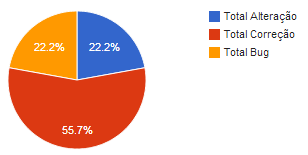
\includegraphics{images/graphic.png}
\end{figure}
\cite{metricas-sao-silvestre}

\subsection{Questão 3}\label{sec:questao-3}
Qual é o número mínimo de profissionais envolvidos para a resolução de cada incidência
\subsubsection{Resposta 3}
O número mínimo de profissionais para a resolução cada incidência, independente qual seu tipo, será de 3 (três) profissionais, sendo eles:

\begin{itemize}
	\item \textit{Programador}: Profissional que realizará a tarefa de correção da incidência encontrada.
	\item \textit{Analista / Testador}: Profissional que irá homologar se a tarefa foi realizada da maneira correta.
	\item \textit{Administrador de Sistemas}: Profissional responsável por atualizar tanto o ambiente de homologação quanto de produção.
\end{itemize}

\subsection{Questão 4}
Qual é o número de horas gasta por cada profissional envolvido no processo para a resolução de uma incidência?

\subsubsection{Resposta 4}
Cada incidência, independente de seu tipo, pode carregar em si uma intrínseca complexidade pois, em muitos casos, os fatores ou dados necessários  para a reprodução do problema são mais complexos de se obter ou simular do que muitas vezes corrigir o problema priopriamente dito.

O programador, com base nas informações de uma incidência, precisa reunir dados para a reproduzir o comportamento informado, corrigir e evidênciar a implementação realizada está de acordo com o comportamento previsto para a funcionalidade proposta.

O analista ou testador, a partir dos dados disponíveis para a reprodução do problema irá verificar a correção realizada, em caso de aprovação, irá para o ambiente de produção, caso contrário, uma nova tarefa será criada para corrigí-la.

O administrador de sistemas, irá atualizar ambos os ambientes, ou seja, quando o programador disponibilizar a correção, esta primeiramente será aplicada em ambiente de homologação e, posteriormente, em produção.

Deste modo, com base em uma média de base histórica, a estimativa para cada profissional será:

\begin{itemize}
	\item \textbf{Programador}: 
		\begin{itemize}
			\item Alteração: 7 horas
			\item Correção: 8 horas
			\item Bug: 12 horas
		\end{itemize}
	\item \textbf{Analista / Testador}: 3 horas
	\item \textbf{Administrador de Sistemas}: 2 horas
\end{itemize}

\subsection{Questão 5}
Qual é o valor da hora de trabalho de cada profissional envolvido no processo de resolução de uma incidência?

\subsubsection{Resposta 5}
De modo a calcular o valor destes profissionais, será utilizado a média salarial entre 2012 e 2013 pago pela empresa responsável pelo projeto. O método utilizado para se obter o valor hora de cada profissional é resultado da seguinte fórmula: 

\begin{itemize}
  \item[] \textbf{$\text{Valor Hora}=\frac{\text{Valor Base} / 30}{8}$}
\end{itemize}

Desta forma, temos a partir da média do salário base o valor hora de cada profissional:

\begin{itemize}
	\item \textbf{Programador}: Salário base: R\$ 4.300,00, salário hora: R\$ 17,92.
	\item \textbf{Analista / Testador}: Salário base: R\$ 5.500,00, salário hora: R\$ 22,92.
	\item \textbf{Administrador de Sistemas}: Salário base: R\$ 6.700,00, salário hora: R\$ 27,92.
\end{itemize}

\subsection{Questão 6}
Qual é a estimativa de horas gastas para a resolução de uma incidência encontrada?

\subsubsection{Resposta 6}
A estimativa de horas gasta por uma incidência é resultado da soma das horas trabalhadas por cada profissional envolvido no processo, sendo assim temos:

\begin{itemize}
	\item Alteração: 12 horas
	\item Correção: 13 horas
	\item Bug: 17 horas
\end{itemize}

\subsection{Questão 7}
Qual é a estimativa do total de horas gastas para a resolução das incidências encontradas?

\subsubsection{Resposta 7}
De acordo com o número de horas estimado anteriormente por incidência, podemos estimar que, para as \alteracoes~incidências de alterações foram gastas 468 horas, para as \correcoes~incidências de correções foram gastas 1274 horas e para as \bugs~foram incidências de bugs foram gastas 663 horas para suas devidas correções.

Portanto, o total de horas gasta com todas as incidências encontradas foi de 2405 horas.

\subsection{Questão 8}
Qual é a estimativa do valor gasto para a resolução de uma incidência encontrada?

\subsubsection{Resposta 8}
A estimativa do valor gasto por uma incidência é resultado da soma do valor hora de cada profissional envolvido no processo, sendo assim, uma incidência específica é resultante da multiplicação do número de horas gastos por cada profissional com seu respectivo valor hora, sendo assim temos:

\begin{itemize}
	\item Alteração: $(7 * R\$~17,92) +  (3 * R\$~22,92) + (2 * R\$~27,92) = R\$~250,04$.
	\item Correção: $(8 * R\$~17,92) +  (3 * R\$~22,92) + (2 * R\$~27,92) = R\$~267,96$.
	\item Bug: $(12 * R\$~17,92) +  (3 * R\$~22,92) + (2 * R\$~27,92) = R\$~339,64$.
\end{itemize}

\subsection{Questão 9}
Qual é a estimativa do valor total gastos para a resolução das incidências encontradas?

\subsubsection{Resposta 9}
De acordo com o valor unitário estimado por incidência estimamos que, para as 39 incidências de alterações foram gastos $R\$~9.751,56$ reais, para as 98 incidências de correções foram gastos $R\$~26.260,08$ reais e para as 39 incidências de bugs foram gastos $R\$~13.245,96$ reais.

Portanto, o valor total gasta com todas as incidências encontradas foi de  $R\$~49.257,60$ reais.

%%%%%%%%%%%%%%%%%%%%%%%%%%%%%%%%%%%%%%%%%%%%%%%%%%%%%%%%%%%%%%%%%%%%%%%%%%%%%%%%%%%
% 4. Considerações finais - o que se pode concluir dos resultados?
%%%%%%%%%%%%%%%%%%%%%%%%%%%%%%%%%%%%%%%%%%%%%%%%%%%%%%%%%%%%%%%%%%%%%%%%%%%%%%%%%%%
\section{Conclusão}
Com base nos fatos citados, podemos observar que o alto número de incidências encontradas através de análise do repositório, bem como do board de gerenciamento do projeto, evidencia que o uso de uma ferramenta como bugtracker seria mais eficaz para gerenciar este tipo de informação e também, afim de facilitar a obteção de futuras métricas concernente a este projeto.

O custo dos bugs e correções somados é equivalente a 9,2 meses de salário bruto de um programador da empresa no período citado. O critério para chegar a este número foi resultado do seguinte cálculo: (custo da correções + custo da bugs) / (salário programador) = (R\$ 26.260,08 + R\$ 13.245,96) / R\$4.300,00 = 9,2.

A implementação de testes unitários faria com que o número de correções encontrado em futuras medições fosse drasticamente menor bem como, seria um fator primordial para a implementação de um processo de integração contínua na empresa.

O uso de integração contínua na empresa faria com que o processo de deploy que, atualmente demora em torno de 2 horas fosse diminuido para em alguns meros minutos, tirando o fator humano interente ao procedimento. Desta forma, o tempo estimado gasto pelos administradores de sistema com o deploy das 176 incidências foram de 352 horas com um custo de R\$ 9.827,84 seria a economia que teríamos para a empresa com tal implementação.

O percentual de bugs em relação a soma dos bugs e correções é de 28,47\%. Isto significa que quase 1 em cada 3 erros não são detectados na fase de testes e sim em produção. Isto evidencia a necessidade de melhor treinamento aos responsáveis pela execução dos testes atualmente ou, a criação de uma equipe independente para tal, visto que, o testador é o próprio analista de negócio, que não possui esta especialidade.

\subsection{Trabalhos Futuros}
Este trabalho poderia ser repetido futuramente com a aplicação das melhorias propostas sugeridas na conclusão deste trabalho afim de levantar novas métricas evidenciando as conclusões obtidas.

Caracterizar as incidências de correções de modo a identificar se esta foi decorrente de falha do desenvolvedor ou problemas de especificação, algo muito recorrente no início do projeto.

Comparar o valor do investimento da implementação dos testes unitários e integração contínua com relação ao valor total das incidências encontradas neste trabalho pela falta destes.\cite{defect-origin-removal}

Fazer uma comparação sobre do número de incidências com valores do mercado ou da literatura, para avaliando com os números da aqui encontrados. Podemos citar que a comparação via incidências/kloc, para projetos com grandes diferenças de linguagem de programação e plataforma, podem gerar resultados imprecisos \cite{loc-metric} \cite{bugs-loc} e que um estudo cuidadoso deve ser feito para chegar-se a um valor que realmente sirva como base para comparação entre eles.

% Faz a criação das referências bibliográficas
\bibliography{Bibliografia}

\end{document}
